\section{Study 3: Evaluation on TypeBoard}

The motivations of study three were two-fold. First, we compared the performance and user experience of the TypeBoard and the ordinary touchscreen keyboard. Second, as we introduced in related work, tactile landmarks on keyboards improve users' typing speed by enabling touch typing, so we investigated the feasibility of TypeBoard plus tactile landmarks in this study. In summary, we evaluated users' typing performance on three settings: (1) ordinary software keyboard, (2) TypeBoard, and (3) TypeBoard plus, which was the TypeBoard plus tactile landmarks.

%实验三的目的有两点:第一,评测TypeBoard的性能,包括在不同的文本输入任务下的输入效率和主观用户体验,baseline是没有防误触算法的触屏键盘。第二,相关工作中我们提到,在防误触触屏键盘上,有望通过加上纹理反馈帮助用户盲打,提高输入效率,本实验探索了这一假设是否成立。

\subsection{Participants}

We recruited 15 participants from the campus (aged from 19 to 26, M = 20.87, SD = 2.42, seven females). All the participants were right-handed and did not take part in the previous studies. They have used software keyboards on smartphones for not less than two years (M = 6.67, SD = 2.06). Eleven participants have ever used software keyboards on tablets.

\subsection{Design and Procedure}

The study followed a within-subject design to compare users' typing speed in three keyboard configurations. The participant sat on an office chair. He could adjust the chair to a comfortable position. The participant typed on the pressure-sensitive touchpad to input words and received visual feedback from the tablet. As figure \ref{fig:study3_illu} shows, there were three settings of the pressure-sensitive touchpad in the experiment as follows:

\begin{enumerate}
	\item{\textbf{Config. 1):} \emph{Ordinary Keyboard.} On the ordinary software keyboard, all contacts on the touchscreen are recognized as keystrokes. Users need to hang their wrists in the air to avoid unintentional touches.}
	\item{\textbf{Config. 2):} \emph{TypeBoard.} TypeBoard is a software keyboard with unintentional touch rejection. The system only recognized intentional touches as keystrokes. Users can rest their hands on the keyboard.}
	\item{\textbf{Config. 3):} \emph{TypeBoard plus.} TypeBoard plus refers to the TypeBoard plus tactile landmarks. To provide tactile landmarks on TypeBoard, we attached 0.05 mm thick stickers on the touchpad to simulate physical keys. There were small bumps on the F and J keys, which is the same as the physical keyboard. Users could align their fingers without visual attention.}
\end{enumerate}

\begin{figure}[!tbh]
	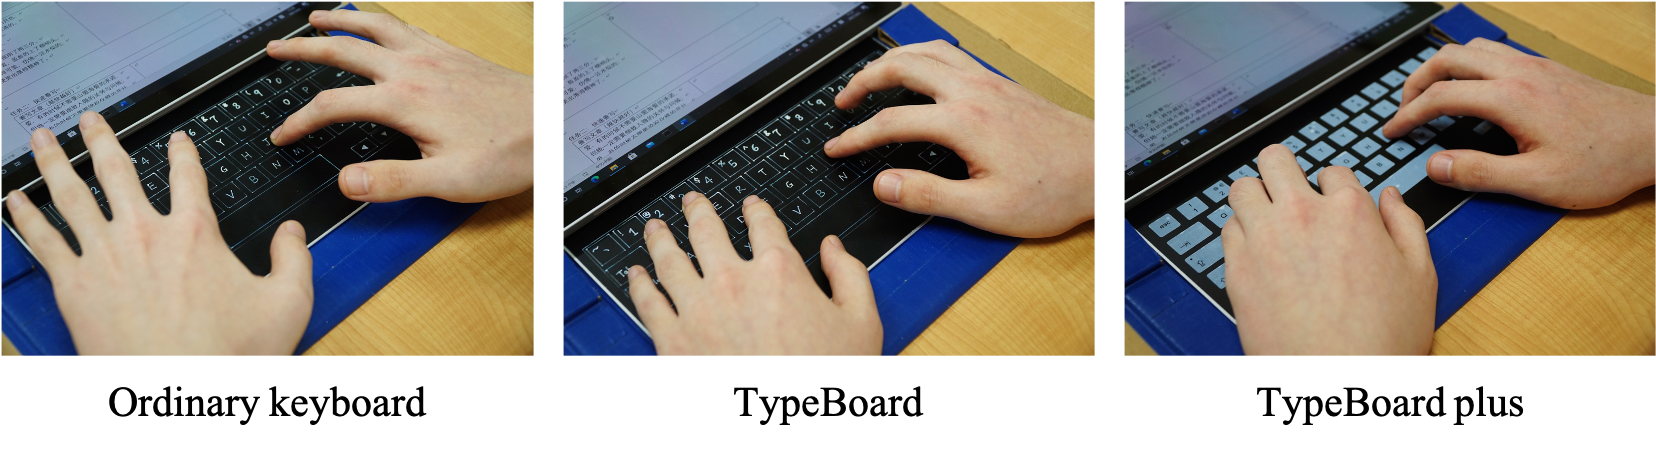
\includegraphics[width=1.0\linewidth]{figures/study3_illu.png}
	\centering
	\caption{图:实验三要对比的三种实验设置,大图是用户实验的整体环境,大图中包含三个小图显示三种键盘配置}
	\label{fig:study3_illu}
\end{figure}

There were five sessions for each of the three keyboard configurations. In each session, participants transcribed a Chinese paragraph in a Microsoft Word document. There were roughly xx Chinese characters in a task paragraph. We randomly selected the task paragraphs in a typing speed measurement website \cite{Website-Typing}. Participants were asked to input as fast and accurately as possible. The transcription task is widely used in text entry researches \cite{2003-Metrics, 2003-Phrase, 2017-Word} to evaluate the ceiling typing speed.  We counterbalanced the order of keyboard configuration using a balanced latin square.
Participants had five minutes to warm up before they used each keyboard. They transcribed a paragraph to get familiar with the keyboard. The task phrases in the training step would not appear in the formal experiment. Participants rested for five minutes between sessions to avoid fatigue. On average, participants spent 90 minutes completing the experiment.

\subsection{Reslut}

A Repeated Measures (RM) ANOVA was conducted for text entry speed, Uncorrected Error Rate (UER), and Corrected Error Rate (CER). The within factors were the keyboard and the session. As UER and CER violated the normalcy, we used the Aligned Rank Transform \cite{2011-Aligned} for correction. If any independent variable had significant effects (p < 0.05), we used Bonferroni-corrected post hoc tests for pairwise comparisons.

\subsubsection{Speed}

We measured text entry speed in Chinese characters per minute (CPM). Participants used Pinyin \cite{Website-Pinyin}, a phonetic spelling system in Roman characters to input Chinese characters. To input a Chinese character, users type the Pinyin of the desired character (2 - 6 letters) and then select the target from a candidate list. Participants can also type the Pinyin of a Chinese word, consisting of two to four Chinese characters, and then select the whole word. In short, the process of inputting a Chinese character/word is similar to inputting an English word with word prediction/correction. We measured typing speed in CPM with this formula:

\begin{equation}
	CPM = \frac{|S|}{T} \times 60
\end{equation}

where |S| is the length of the transcribed paragraph in characters (including punctuation), and T is the completion time, i.e., the elapsed time in seconds from the first intentional touch to the last one. All the time consumption, including the time of candidate selection, was taken into account.

%我们使用的是中文输入法,我们所统计的量是中文字/分钟,公式是,当用户输入数字或字母时,其速度不纳入统计范围。我们测试了五种不同的输入任务,值得注意的是,只有transcription任务中的输入速度比较符合用户的ceiling speed,而在其它任务中,完成任务的时间包含了用户思考的时间和键鼠切换的时间。

\begin{figure}[!tbh]
	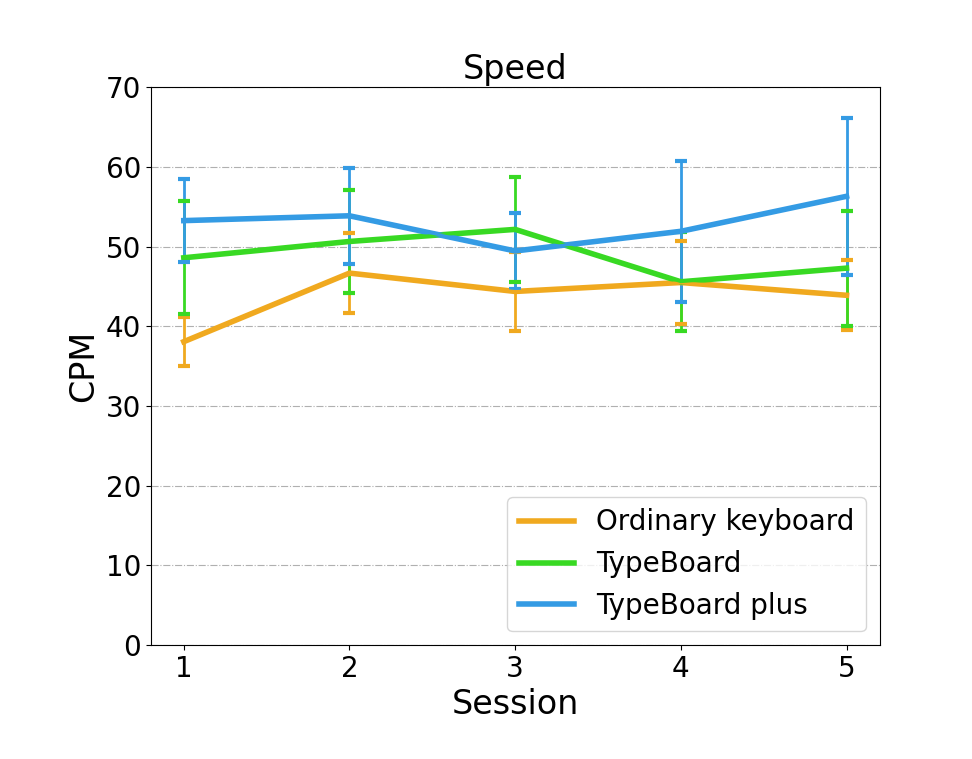
\includegraphics[width=0.6\linewidth]{figures/speed.png}
	\centering
	\caption{Text entry speed of the three keyboards over sessions. Error bars indicate 95\% confidence interval.}
	\label{fig:speed}
\end{figure}

Figure \ref{fig:speed} shows the users' typing speeds over sessions. There is no significant effect of session on speed ($F_{4,56}=1.76,p=.15,\eta_p^2=0.11$). The result indicates that the learning costs of the three keyboards were low. Participants reached the ceiling performance after a five-minute training. Keyboard has a significant effect on speed ($F_{2,28}=26.76,p<.001,\eta_p^2=0.66$). Pair-wise comparisons show significant differences between all the keyboard pairs: ordinary keyboard vs. TypeBoard ($p<.005$), ordinary keyboard vs. TypeBoard plus ($p<.001$), and TypeBoard vs. TypeBoard plus ($p<.005$). The participants' average typing speed on the ordinary keyboard was 43.71 CPM (SD = 6.52). The typing speed on the TypeBoard was 48.87 CPM (SD = 10.14), outperforming the ordinary keyboard by 11.78\%. The typing speed on the TypeBoard plus was 52.97 CPM (SD = 9.85), outperforming the ordinary keyboard by 21.19\%. Results show that the TypeBoard improves the efficiency of the touchscreen keyboard.

\subsubsection{Error rate}

We used two metrics to measure text entry accuracy: (1) Uncorrected Error Rate (UER) - text entry errors that remain in the transcribed string. UER is the number of uncorrected erroneous Chinese characters divided by the number of correct and erroneous characters. (2) Corrected Error Rate (CER) - text entry errors that are fixed (e.g., backspaced) during entry. CER is the number of corrected erroneous Chinese characters divided by the number of correct and erroneous characters. The corrections of Pinyin while inputting a word were not taken into account of CER. As UER and UER violated the normalcy, we used the Aligned Rank Transform for nonparametric factorial analysis \cite{2011-Aligned}.

\begin{figure}[!tbh]
	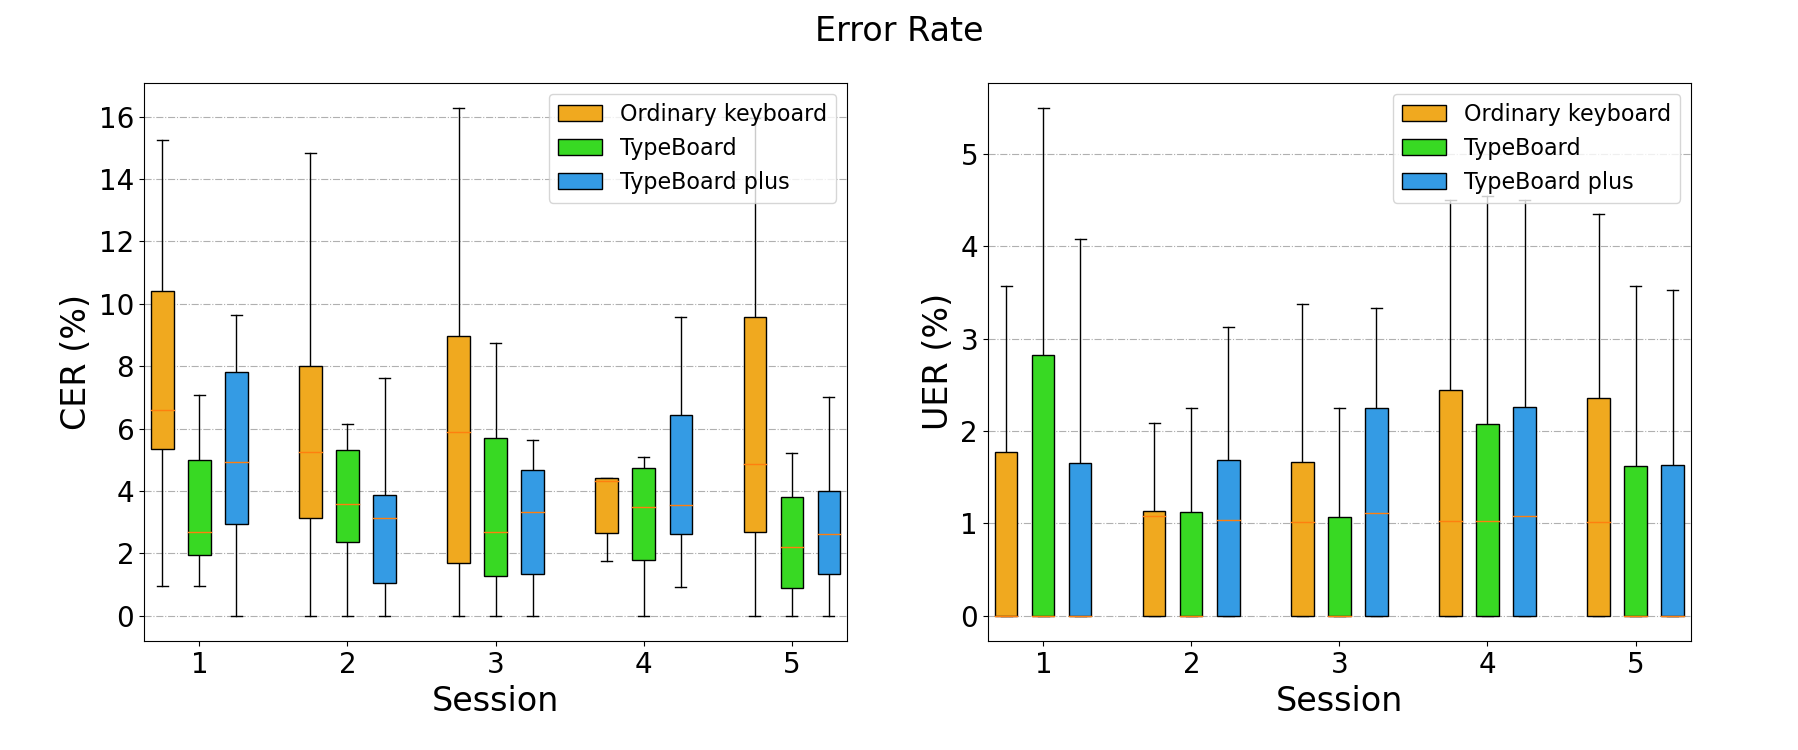
\includegraphics[width=1.0\linewidth]{figures/error_rate.png}
	\centering
	\caption{Uncorrected error rates and Corrected error rates of the three keyboards over sessions.}
	\label{fig:error_rate}
\end{figure}

Figure \ref{fig:error_rate} shows the CER and the UER over sessions. There is no significant effect of session on CER ($F_{4,56}=1.01,p=.39$). Keyboard has a significant effect on CER ($F_{2,28}=9.49,p<.005$). Pair-wise comparisons showed significant differences between the following keyboard pairs: ordinary keyboard vs. TypeBoard ($p<.01$), and ordinary keyboard vs. TypeBoard plus ($p<.005$). The average CERs of the ordinary keyboard, TypeBoard, and TypeBoard plus were 6.66\% (SD = 4.42\%), 4.58\% (SD = 3.58\%), and 4.21\% (SD = 2.58\%).
There is no significant effect of session ($F_{4,56}=0.41,p=.71$) or keyboard ($F_{2,28}=0.001,p=.998$) on UER. The average UERs of the ordinary keyboard, TypeBoard, and TypeBoard plus were 1.29\% (SD = 1.67\%), 1.28\% (SD = 1.38\%), and 1.28\% (SD = 1.16\%).
Results show that the TypeBoard reduces the probability of making a typo compared with the ordinary keyboard. This is the main reason the TypeBoard improves the typing speed of the touchscreen keyboard. The TypeBoard plus does not reduce the probability of making a typo compared with the TypeBoard. Thus, there are other reasons for faster typing on the TypeBoard plus.

%在中文输入法中,CER可能会比其它语言的输入法更多,这是因为用户可能会利用词语的联想功能来打一个汉字,然后把后面那个字删掉。

%Figure 14 shows the UER and the CER over five days. There is no significant effect of model or day on UER. The average UER was 1.17% (SD = 1.02%) for the general model and 1.50% (SD = 1.40%) for the personal model. There is no significant effect of the model on CER. The days have a significant effect on CER (F4,56 = 6.84,p < .005). Pair-wise comparisons showed significant differences between the following day pairs: 1-3(p<.005), 1-4(p<.05), 1-5(p<.005), 2-3(p<.05) and 2-5(p<.05). On day 5, the average CER was 3.22% (SD = 2.92%) for the general model and 2.92% (SD = 1.65%) for the personal model. That is, participants made corrections once every 30 words with both of the models.

\subsubsection{Time components}

Time components.

\begin{figure}[!tbh]
	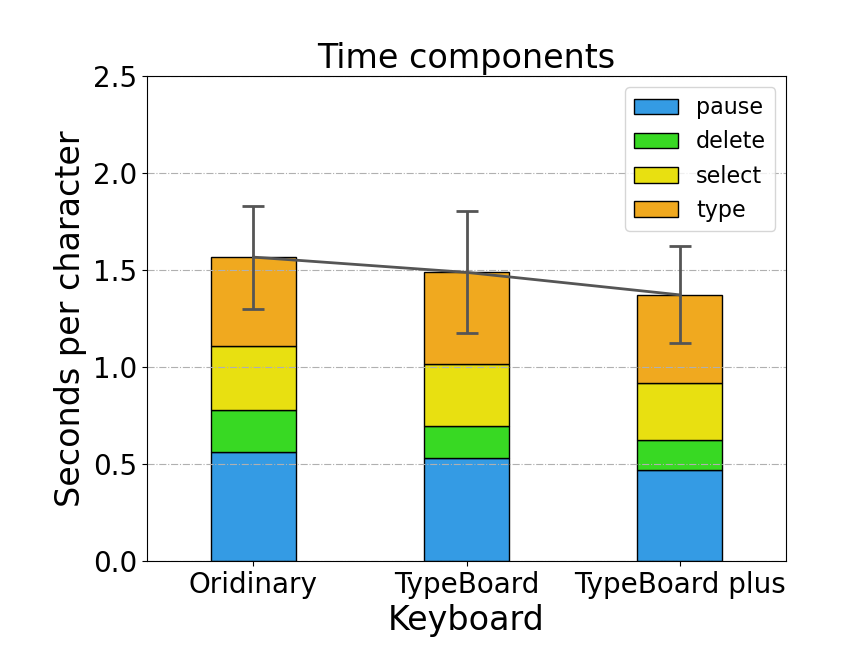
\includegraphics[width=0.6\linewidth]{figures/time_components.png}
	\centering
	\caption{Time components.}
	\label{fig:time_components}
\end{figure}

\subsubsection{Unintentional touches}

For the three configurations ordinary keyboard, TypeBoard and TypeBoard plus, the proportions of unintentional touches were xx.xx\%, xx.xx\% and xx.xx\% respectively.

English.

为了方便计算,我们在上述统计中假设算法100\%正确预测了点击的有意性。

统计发现,显著性影响。

讨论造成显著性的原因。

在实验三中,TypeBoard上的误触与实验二相比显著降低,我们认为,这是任务不同造成的。在誊写这种快速输入的任务下,用户在普通触屏键盘和TypeBoard上都没有必要将手指休息在键盘上。但在TypeBoard+tactile设置下,用户在誊写任务下仍然引发了大量的“误触”,这暗示,用户可能并不只是将手指休息在触屏上,而是尝试利用触屏上的纹理来对齐他们的手指,从而达到部分的盲打。

\subsubsection{Touch position}

%Figure xx illustrates the multiple finger resting behavior through point clouds. The distribution seems optional on the ordinary TypeBoard, and seems regular on the TypeBoard plus tactile landmarks. xx.x\% of the resting touchpoints laid on the second row of keys on the TypeBoard with landmarks, which has an significant difference (F, p) from the ordinary TypeBoard (xx.x\%). This indicates that users leveraged the tactile landmarks to align their fingers.
%【图:用户在multiple finger resting时的手指点云,TypeBoard with/without landmarks】

Figure xx shows the distribution of intentional touchpoints over keyboard configurations. We used xxx to cluster the point cloud of each key. xxx shows that the point cloud obeyed the 2D Gaussian distribution (F, p). The average standard deviation of the distributions were xx.x mm (SD=), xx.x mm (SD=) and xx.x mm (SD=). RM-ANOVA shows that the keyboard has a significant effect on users' touching accuracy (F, p). Users typed more accurately on the TypeBoard plus landmarks compared with the regular keyboard (p) and the TypeBoard (p). The analysis of touch position shows that users aligned their fingers on the TypeBoard with tactile landmarks, which improved their typing accuracy.

【图:各实验设置下用户有意点击点云】

\subsubsection{Subjective Rating and Feedback}

English.

物理负担(疲劳程度),心理负担,主观输入速度,主观输入准确率(误触准确率,而非选词准确率)。

\subsection{Discussion}

\subsubsection{TypeBoard vs. Regular Keyboard}

Compared with regular touchscreen keyboards, the TypeBoard has the advantages of avoiding fatigue and improving subjective user experience.

(1)避免疲劳。TypeBoard用户在誊写任务的每100次打字行为中,系统就会阻止xx.x次多指休息行为和xx.x次小鱼际点击。实验二表面,TypeBoard在其它需要更多键鼠切换或者思考的文本输入任务下,所阻止的多指休息次数会更多(xx.x 每100次点击)。结果表明,用户在TypeBoard上会主动地利用可以将手指和手腕休息在touchscreen上的特性。而且在用户的主观反馈当中,用户也表示TypeBoard显著地降低了他们的疲劳程度。
(2)主观用户体验。TypeBoard在主观输入速度、主观输入准确率等方面都显著优于普通键盘。这说明TypeBoard可以提高用户体验。

我们推断,TypeBoard的优势主要在降低错误率,和避免疲劳。

\subsubsection{TypeBoard vs. TypeBoard plus}

English

TypeBoard plus 是我们设想中的一种软键盘形态,即利用可变形触屏[xx]或者添加layout[xx]的方法来达到提供触觉landmarks的目的。我们发现,TypeBoard plus不仅能够降低疲劳、提高用户体验,还能够显著地提高软键盘上的文本输入速度,将输入速度提高xx.x\%。输入效率提高的主要原因是用户可以在TypeBoard plus中align fingers,从而实现盲打。

我们推断,TypeBoard的优势主要在盲打。
